\section{Design av l\o sningen}

	\subsection{Overordnet design (Holger)}
	
		\begin{figure}[h]
		\centering
		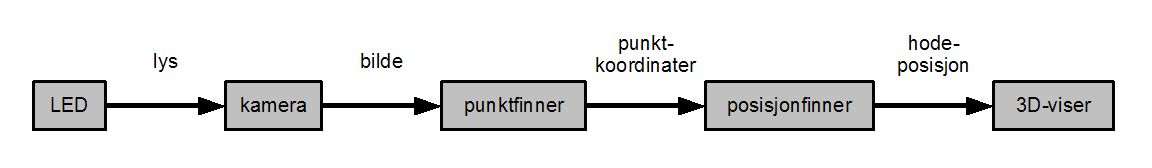
\includegraphics[width=\textwidth]{graphics/main_design.png}
		\caption{Overordnet design}
		\label{fig:main_design}
		\end{figure}
		
		Den overordnede designen er en pipeline som begynner med lys fra LEDs og ender opp med visning av en 3D-scene. Figur \ref{fig:main_design} illustrerer dette. Vi ser at alt begynner med infrar\o de LEDs som er festet p\aa \space hodet til brukeren. Disse sender lys som filmes av kameraet. Bildene fra kameraet leses av kode som finner punktene p\aa \space bildet som senteret til hvert filmet LED. Disse koordinatene sendes til kode som bruker dem til \aa \space beregninge posisjonen til hodet. Denne posisjonen sendes til kode som viser en 3D-scene p\aa \space skjermen, hvor synsvinkelen passer posisjonen til hodet.
	
	\subsection{Design av LED-headset (Jon)}
	
		
	
	\subsection{Design av punktfinneren (Holger)}
	
			
	\subsection{Design av posisjonsfinneren og 3D-viseren (Vegar)}
	
		
	
\section{Implementasjon av l\o sningen}

	